In the case of SKA, different solutions for time transfer were analyzed. For instance, GPS devices provide a reference frequency (10-50 MHz), a PPS signal and a serial code to provide the time (typically based on the NMEA protocol). This approach is widely used in many systems that require accurate synchronization (since various instrumentation can be easily connected to different GPS receivers) but it is sensitive to jamming issues. Alternatively and thanks to the packet networks popularity, the timing protocols are little by little imposing as main solution for time transfer over the network. Low performance protocols as Network Time Protocol (NTP), the protocol used in Internet to synchronize the computers through the network), \cite{ntf:ntp_std} are widely used while for industrial applications the preferred protocol is the IEEE-1588v2 (known as Precision Time Protocol or PTPv2) \cite{ieee:ieee1588_std} \cite{itu:TG8275_1_Y_1369_1}. IEEE-1588v2 is an industrial evolution of NTP, characterized by the utilization of hardware time-stamping mechanisms that significantly improved time synchronization accuracy. Typically, NTP provides about 1ms synchronization accuracy while PTPv2, working on very well designed time-aware networks is able to achieve about 50ns synchronization accuracy. 
Although previous approaches are quite accurate, they are not appropriated to fulfill the specifications of the 2ns requirement associated to the SKA1 telescope. As alternative solution, the utilization of the White Rabbit (WR) protocol has been proposed because it is an evolution of IEEE-1588v2 protocol and able to distribute an absolute time reference with an accuracy of 1ns. Equipment located at each endpoint delivers a 1PPS signal with its edge aligned to the start of the UTC second. Therefore, each telescope can then be phased up by observing the white light fringe on one or more bright, compact sources.

The White Rabbit (WR) technology is an international, collaborative project started at CERN in 2009, and then joined by other laboratories and companies. It was born as replacement technology for the timing system at CERN, but thanks to its versatility, improved performance, compared to the alternatives, and open nature of the project, it was quickly adopted by other scientific institutions. There is also a strong interest in private companies to extend WR in the industrial world such as Seven Solutions \cite{sevensols:wr}. Furthermore, from its very early stages, WR was launched as an open Sw/Hw initiative with sources available at the Open Hardware Repository \cite{ohwr:repo}. This encouraged different companies and research institutions to openly collaborate in its development.

The WR protocol extends Precise Time Protocol version 2 (PTPv2) with extra messages, proposed to be included in the new PTP release (PTPv3) as High Accuracy profile. Its main goal is to provide a synchronization accuracy better than 1ns and precision in the scale of picoseconds. The major improvements introduced in the WR protocol address weak aspects of the PTPv2: the limitation in the phase difference measurements to one period of the system clock; and the assumption of symmetry between the transmission and reception paths. It inherently performs self-calibration over optical fiber links and it is capable of distributing time to a very large number of devices with very small degradation. Nevertheless, this technology in the origin was not designed to address large distances or provide embedded nodes with monitoring and dependable mechanism. Although SKA1 is working on improving both issues, we particularly focus on this contribution on providing a novel platform capable disseminate the PPS signal ad with flexibility and dependability characteristics.  

%\textst{WR is based on other technologies such as the L1 synthonization of Synchronous Ethernet (SyncE), an extension of PTPv2 (WR-PTP) and additional phase %alignment techniques. The L1 synthonization is responsible for transmitting the master clock inside the data stream in order to slave devices can recover it from %the network and adjust their oscillator frequencies to follow the reference clock.} 

%\textsterling{WR also uses additional phase alignment techniques as the Digital Dual Mixed Time Difference (DDMTD) that is a module responsible for measuring the %phase between two clocks. This information is used to change the frequency of the local oscillator for the synchronization process.}

The WR synchronization mechanisms include the following elements:

\begin{itemize}
	\item {Frequency synchronization (synthonization): It uses L1 synthonization of Synchronous Ethernet (SyncE) to encode the clock signal in the data carrier. It is responsible for recovering the clock from the network and to adjust local oscillator to follow it.}
	\item {Phase synchronization: The physical clock of a node is retransmitted to the master element and viceversa so that master can compare the phase of this signal (coming from the slave) with its own phase. The deviation should be equal to the propagation time of the signal through the fiber. The master can determine the phase difference between its own clock and the network recovered one and send back this information to the slave. The phase measurement is performed by an IP core known as Digital Dual Mixed Time Difference (DDMTD) present in the gateware design.}
	\item {Time synchronization: It is implemented by PTPv2 protocol and provides a global notion of time to the entire network. WR also takes into account the asymmetries in the propagation time due to the utilization of different wavelengths in the same fiber link improving the accuracy of standard PTP protocol.}
\end{itemize}

%%Internal oscillators of the WR devices run locked to the master's reference clock of the network, allowing precise phase difference 
%%measurements between the master clock and the slave clock. 

WR implements mechanisms to ensure deterministic and reliable data transfer between a thousand of nodes connected with  optical fiber links up to 10 km. However, it can easily be extended up to 50 km without significant degradation and up to 120 km without the needs of optical amplification. A typical WR network is arranged in tree topology. This is very common in timing networks where time reference is propagated downlink from a root device, known as Grand Master, that can be connected to a very stable clock, such as an atomic clock or a GPS receiver. Currently, new network topologies are under-study in WR to add some mechanisms for improving the redundancy and security. An example of this research is \cite{jlgutierrez-paper-redundancy} that incorporates the Transparent clocks (TC) to WR protocol and allows implementing redundancy protocols such as HSR or PRP to ensure the data delivery and reception in critical applications.

The intermediate levels of the network spread the timing packets to the final nodes and are composed of other devices such as WR Switches, WR-ZEN or WR-LEN that have several ports and can behave as PTPv2 Boundary Clocks (BC). Their different ports are divided on two types: one of them is the slave (uplink) and connects to the upper layer and the other ports are masters (downlinks) and they are charged to propagate the synchronization to the next level of the hierarchy. The nodes of the last level of the network are known as Slave devices that recover the clock signal of the link and synchronizes their local oscillators to provide synchronization for a specific application or facility.

\begin{figure}[H]
	\centering
	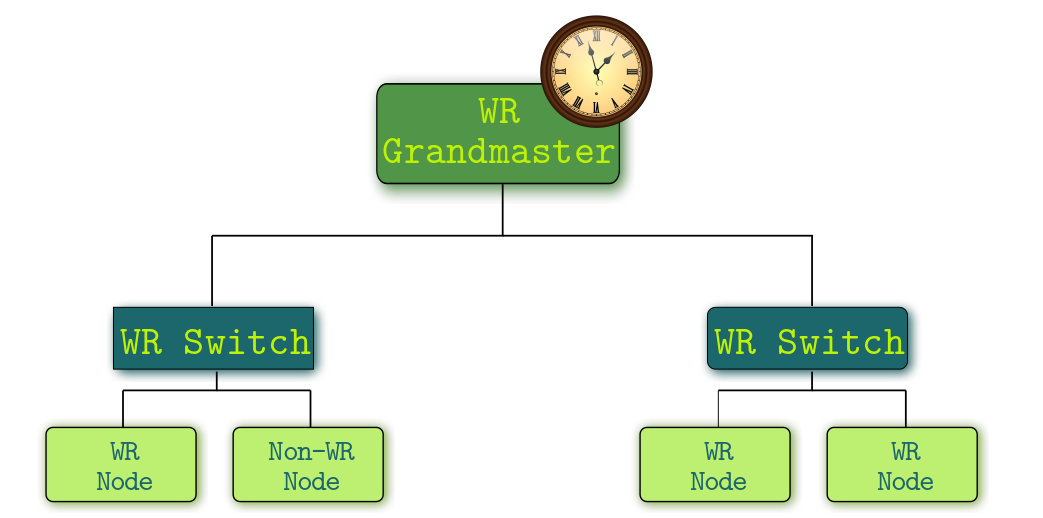
\includegraphics[scale=0.4]{img/wr_hierarchy}
	\caption{The WR network is a tree hierarchy where the root node is the Grand Master that is responsible for distributing the reference time signals. The intermediate elements are WR Switches that acts as Gigabit Ethernet switchers and as Boundary clocks propagating the time signals from the upper layers of the network. Finally, the leaf nodes are known as nodes and its main purpose is to provide timing to another specific application.}
	\label{fig:wr_hierarchy}
\end{figure}

%\missingfigure{Añadir figura para mostrar la topología WR}

WR is designed to be fitted in a Field Programmable Gate Array (FPGA) device due to its flexibility to use in designs in a continuous development state. The source code is mainly written in Hardware Description Languages (HDLs) such as VHDL or Verilog. Moreover, there are several platforms that can implement WR that ensures the vendor-independent feature of WR. The most extended vendor in WR world is Xilinx, some examples of devices using Xilinx's FPGAs are the SPEC board \cite{ohwr:spec} and the WRS \cite{ohwr:wrs}. The other vendor used in WR is Altera. Some examples of boards could be found in \cite{cesar-altera-wr}. The main Intellectual Property (IP) block is the WR PTP core (WRPC) for WR nodes and the Real Time Subsystem (RTS) for WR switches. The most common WR nodes are based on carrier boards such as SPEC or SVEC and can be plugged in a PCIe/VME socket of a conventional PC. Some WR nodes have a standalone mode but in this case they can not benefit of high level features usually provided by a PC CPU.

The WR Zynq Embedded Node (WR-ZEN) is a new generation board that includes a Xilinx Zynq System-on-Chip (SoC). The Zynq SoC is composed of a FPGA and a hard ARM dual core microprocessor that can run an application that controls the hardware directly or a standard Operating System such as Linux that can host many different kind of processes at the same time. The WR-ZEN has been proposed to be used in the SKA project to implement the PPS distribution system.

Next sections will present the main possible WR contributions for SKA time dissemination: WR Precision Time Protocol for clock propagation and the generation of PPS signal. 
